\chapter{Introduction}\label{intro}
Write your introduction in this section.
Use sections and sub sections to organize the chapters.

\section{Thesis}
The introduction of a thesis serves as a crucial foundation for the research presented. It typically begins by introducing the topic and providing essential background information to contextualize the study. This section outlines the research problem or question, highlighting its significance and relevance within the existing body of knowledge. Additionally, it specifies the objectives of the research, detailing what the study aims to achieve and how it will be conducted. The introduction often concludes with a roadmap that outlines the structure of the thesis, guiding the reader through the upcoming chapters. Overall, the introduction is designed to engage the reader, establish the importance of the research, and clearly articulate the focus and scope of the study.
\section{Project}
The introduction of a project outlines the essential details and context for the work being presented. It typically begins with a brief overview of the project’s topic, followed by background information that situates the project within a broader framework. This section explains the motivation behind the project, including why the chosen theme is significant and what inspired the research. Additionally, it often highlights specific objectives and goals, providing a clear statement of what the project aims to achieve. The introduction may also include a summary of the resources used and the timeline for execution, setting expectations for the reader regarding the project's structure and content. Overall, it serves to engage the audience and establish a foundation for understanding the project's relevance and scope.
\subsection{Subsection}
Sub-subsections are numbered as given above and included as a third level of text. 
\subsubsection{Sub-subsection}
If necessary split your subsections into further sub-subsections.

\section{Guideline for web based projects}
For web based projects, follow the guidelines.
After introductory paragraph go with ther following sections
\begin{itemize}
    \item Project Motivation and Target User Groups
    \item Similar Products and their features
    \item Features of our product as Requirements:
\end{itemize}

\section{Project Motivation and Target User Groups}
First paragraph: Write why did you choose this project.

Second paragraph: Write who will use this project. How will they be benefit using your project.

\section{Similar Products and their features}
Write an introductory paragraph first. In this section you will create several subsections, each outlining one product and its features.
\subsection{Similar Product 1}
Write description of this product in a single paragraph. 

\subsection{Similar Product 2}
Write description of this product in a single paragraph. 
You can also use photographs of some products if you like. An example of how you can add screenshots of similar products is given below:
\begin{figure}[h]
    \centering
    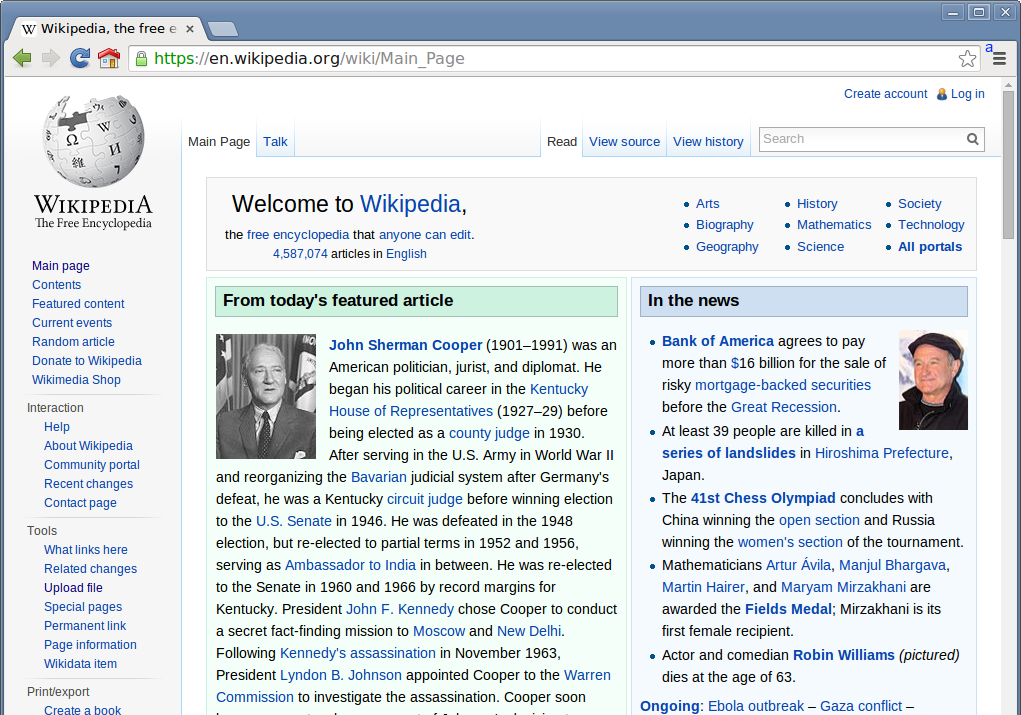
\includegraphics[width=0.7\textwidth]{figures/demoFigure1.png}
    \caption{A sample Wikipedia page.}
    \label{fig:wikiDemo}
\end{figure}
Formatting figures: Always keep the figures center and avoid overstretching the figures. Ideally figures should encompass less that 70\% of text width. 
All figures should be accompanied by relevant caption. Also, all figures must be referenced withing the text. For example the figure \ref{fig:wikiDemo} is a demo page of Wikipedia.
When giving screenshot of others product or using figures of others, you MUST provide proper citation.

\subsection{Similar Product 3}
you have more similar products, add them here.

\subsection{Similar Product 4}
you have more similar products, add them here.


\section{Features of our product as Requirements:}
In this section include both functional and non-functional requirements of your product.

\subsection{Functional Requirement:}
Write all functional requirements as a list.

\subsection{Non-functional Requirement:}
Write all non-functional requirements as a list.

Note that, you will have a separate chapter for requirement analysis. However, you should include a summary of product requirements in the introduction chapter itself.